\chapter{Results}
Some of the results presented here are compared with output from FREYA (Fission Reaction Event Yield Algorithm). 
FREYA was developed by the collaborative efforts of researchers from Lawrence Berkeley National Laboratory,  Lawrence Livermore National Laboratory, Los Almost National Laboratory, and University of Michigan Nuclear Engineering.
It has been included in MCNP since version 6.2 .
All analysis performed on the measured data also applied to the data output by FREYA, with the exception of accidental subtraction.
This includes the normalization to uncorrelated neutrons and the weighting procedures that are described in section~\ref{Analysis}.
 
The most recent release of FREYA, version 2.0.3, does not model photofission directly, but instead uses a neutron-induced fission model to approximate photofission~\cite{FREYA_photofission}.
For a given nucleus with Z protons and A total nucleons, the code selects the neutron-induced fission model for the Z(A-1) nucleus, and chooses an incident neutron energy such that the compound ZA nucleus will have an excitation energy, relative to the ground state of ZA, that is equal to the energy of the incident photon.
All model parameters, such as level density and partition parameters, were set to their default values for neutron-induced fission.
FREYA was told to use the fission fragment mass distribution $Y(A)$ and the average total kinetic energy $\langle$TKE$\rangle(A)$ from the photofission of $^{238}$U, which was taken from the work discussed in ref~\cite{2017Krishichayan}.

In ref~\cite{Talou2018}, the authors warn that using FREYA in this way to model photofission is only an approximation and could lead to incorrect results.
Nonetheless, the approximation is presented here because it is the only photofission model available to the authors of the present work.

\section{correlation}
Figure~(TODO) shows the measured $\theta_{nn}$ distribution from the photofission of $^{238}$U for various ranges of mean neutron energy compared to a FREYA simulation.

\section{Correlation of $\theta_{abs}$}
While these results are consistent with the effect of the kinematic focusing of the neutrons due to the recoil of the fission fragments, the data show a marked decrease in the two-neutron opening angle correlation in the region from about 165 to 180 degrees, which is well-pronounced in Fig.~\ref{fig:SPDPNormalization} and can also be seen in Figs~\ref{fig:FinalDUResult} and~\ref{fig:theta_abs_two_neutron}.
This feature is not evident in previous work on spontaneous and neutron induced fission.
As previously discussed, photofission differs from spontaneous and neutron induced fission in that the fission fragments for the photon induced reaction exhibit an asymmetry in their angle of emission, with the most likely orientation of the fission axis lying perpendicular to the direction of the incident photon.
With this in mind, the following series of angular cuts were made on the data.
Fig.~\ref{fig:theta_abs_LEGO} shows the distributions of absolute opening angles of the two-neutron events for three different cuts on the value of the two-neutron opening angle.
For two-neutron opening angles between 120 and 160 degrees, there is an increased preponderance of both neutrons being emitted around 90 degrees, consistent with the interpretation of kinematic focusing of neutrons coming from fission fragments which are themselves being emitted preferentially at 90 degrees.
However, in the opening angle region where the two-neutron correlation is reduced, from about 160 to 180 degrees, this feature is less prominent.

Furthermore, if one plots the opening angle distributions for the case in which at least one neutron is emitted perpendicular to the incident photon versus the case in which neither neutron is emitted perpendicular to the incident photon (Fig.~\ref{fig:theta_abs_two_neutron}), one sees that the two-neutron correlation is greatly reduced at 180 degrees in opening angle when at least one of the neutrons is emitted along the preferred fission axis.

These data are consistent with two possible explanations.
First, it is possible that there is a decrease in neutron emission along the fission axis.
Second, the neutrons may indeed be emitted isotropically in the rest frame of the fission fragment, but one fragment essentially shadows the neutrons emitted from the other fragment, either through absorption or scattering.
A definitive interpretation of this decreased two-neutron correlation for large opening angles in photo-fission requires further study.

\begin{figure}
    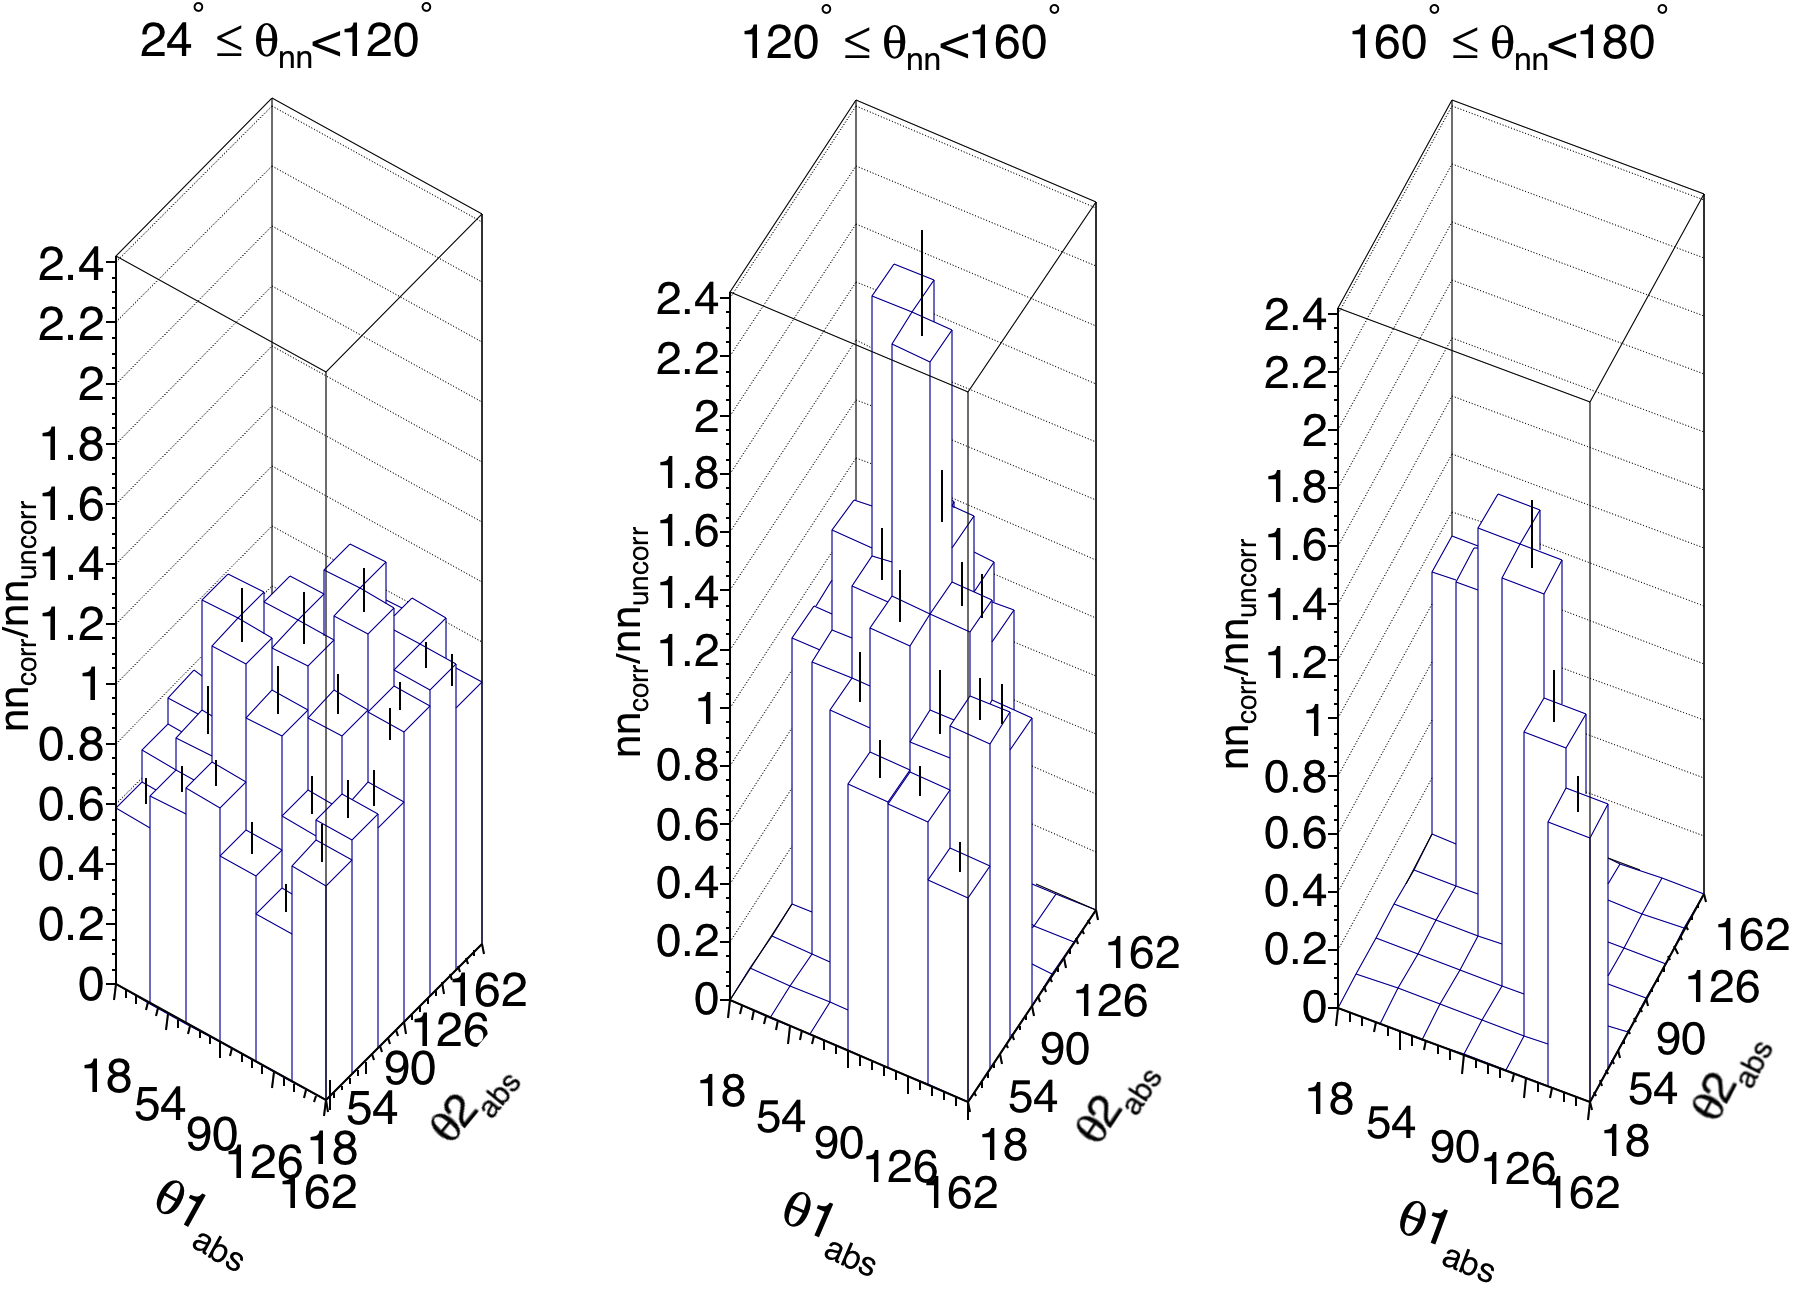
\includegraphics[width = 0.9\textwidth]{Content/Results/theta_abs_LEGO.png}
    \caption{Correlation is shown between the angles of each neutron with respect to the incident photon beam, denoted by $\theta 1_{abs}$ and $\theta 2_{abs}$.
    Empty bins exist because of incomplete $\theta_{abs}$ coverage.}
    \label{fig:theta_abs_LEGO}
\end{figure}
\begin{figure}
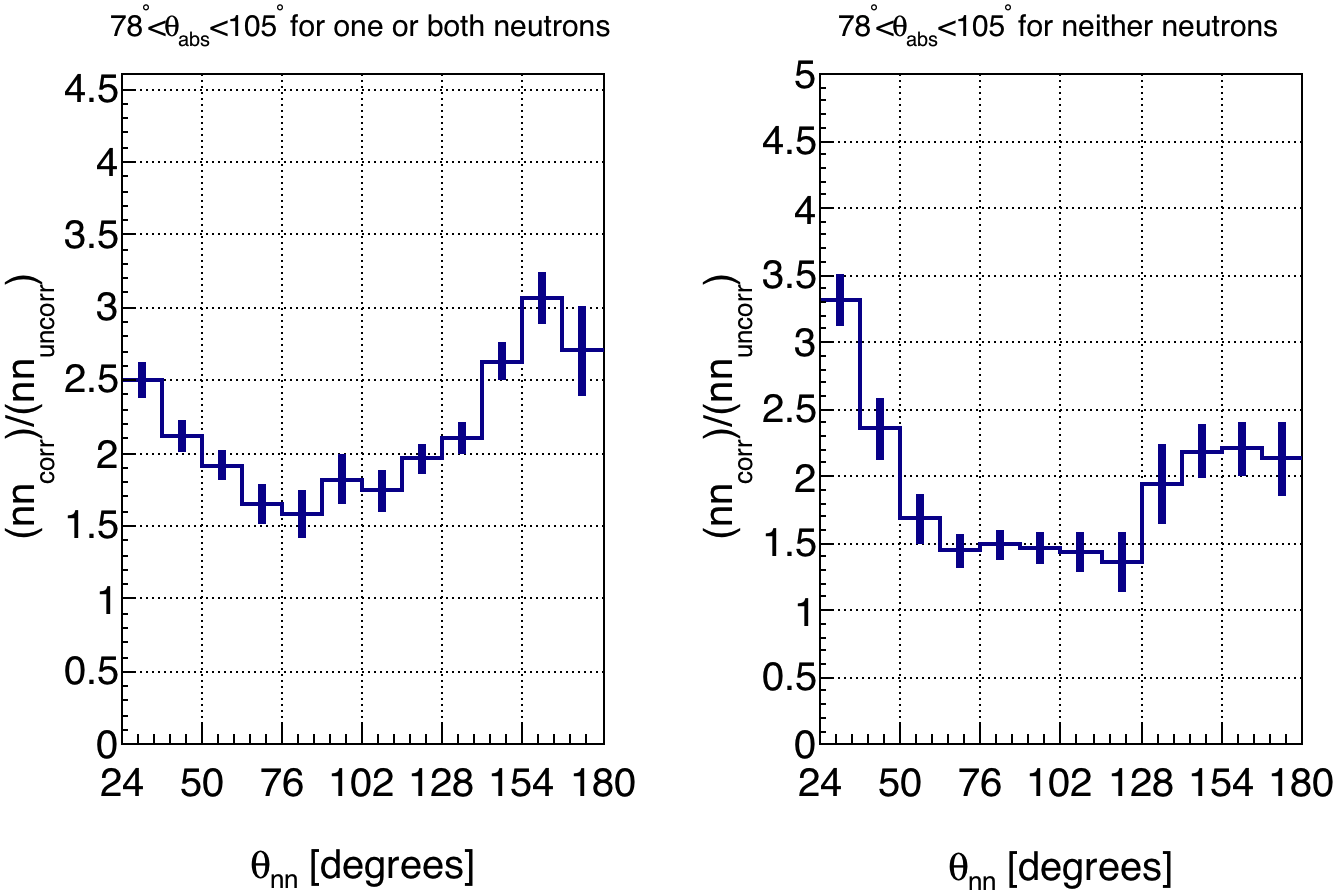
\includegraphics[width=0.9\textwidth]{Content/Results/theta_abs_two-neutron.png}
\caption{Requiring that at least one of the coincident neutrons be emitted nearly perpendicular to the photon beam (left) produces an opening angle distribution that is different from that produced when requiring that both neutrons are emitted nearly parallel to the photon beam (right).}
\label{fig:theta_abs_two_neutron}
\end{figure}

\FloatBarrier 
